%-------------------------------------------------------------------------------
%-------------------------------------------------------------------------------
\begin{frame}\begin{center}
		\LARGE\textbf{True returns}
\end{center}\end{frame}
%-------------------------------------------------------------------------------
%-------------------------------------------------------------------------------
\begin{frame}
Suppose their is uncertainty about net earnings conditional on $s$ and actual lifetime earnings for someone with $s$ years of schooling are:

\begin{align*}
Y_s = \left[\sum^T_{x = 0}(1 + r)^{-1} Y(s, x)\right]\epsilon_s
\end{align*}
\end{frame}
%-------------------------------------------------------------------------------
%-------------------------------------------------------------------------------
\begin{frame}
We assume that $\E_{s - 1}(\epsilon_s) = 1$ and define expected earnings associated with schooling $s$ conditional on current schooling $s - 1$,

\begin{align*}
\bar{Y}_s = \E_{s - 1}(Y_s)
\end{align*}
\end{frame}
%-------------------------------------------------------------------------------
%-------------------------------------------------------------------------------
\begin{frame}
The decision problem for a person with $s$ years of schooling given the sequential revelation of information is to complete another year of schooling if

\begin{align*}
Y_s \leq \frac{E_s(V_{s+1})}{1 + r}.
\end{align*}

\end{frame}
%-------------------------------------------------------------------------------
%-------------------------------------------------------------------------------
\begin{frame}
So the value of schooling level $s$, $V_s$, is

\begin{align*}
V_s = \max\left\{Y_s, \frac{E_s(V_{s+1})}{1 + r}\right\}
\end{align*}
for $s \leq \bar{S}$. At the maximum schooling level, $\bar{S}$, after all information is revealed, we obtain $V_{\bar{s}} = Y_{\bar{s}} = \bar{Y}_{\bar{s}}\epsilon_{\bar{s}}$.

\end{frame}
%-------------------------------------------------------------------------------
%-------------------------------------------------------------------------------
\begin{frame}
The endogenously determined probability of going on from school level $s$ to $s + 1$ is

\begin{align*}
p_{s + 1, s} = \Pr\left(\epsilon_s \leq \frac{E_s(V_{s + 1})}{(1 + r) \bar{Y}_s}\right),
\end{align*}
where $E_s(V_{s + 1})$ may depend on $\epsilon_s$ because it enters the agent's information set.
\end{frame}
%-------------------------------------------------------------------------------
%-------------------------------------------------------------------------------
\begin{frame}
The average earnings of a person who stops at schooling level $s$ are

\begin{align*}
E_{s - 1}(V_s) & = \underbrace{(1 - p_{s + 1, s}) \bar{Y}_s E_{s - 1}\left(\epsilon\mid \epsilon \ge \frac{E_s(V_{s + 1})}{(1 + r)\bar{Y}_s)}\right)}_{\text{direct return}} \\
 & + \underbrace{p_{s + 1, s} \left(\frac{E_{s - 1}(V_{s + 1})}{1 + r}\right)}_{\text{option value}}.
\end{align*}
\end{frame}
%-------------------------------------------------------------------------------
%-------------------------------------------------------------------------------
\begin{frame}
\begin{figure}[htp]\centering
\caption{Option values and uncertainty}
\scalebox{0.35}{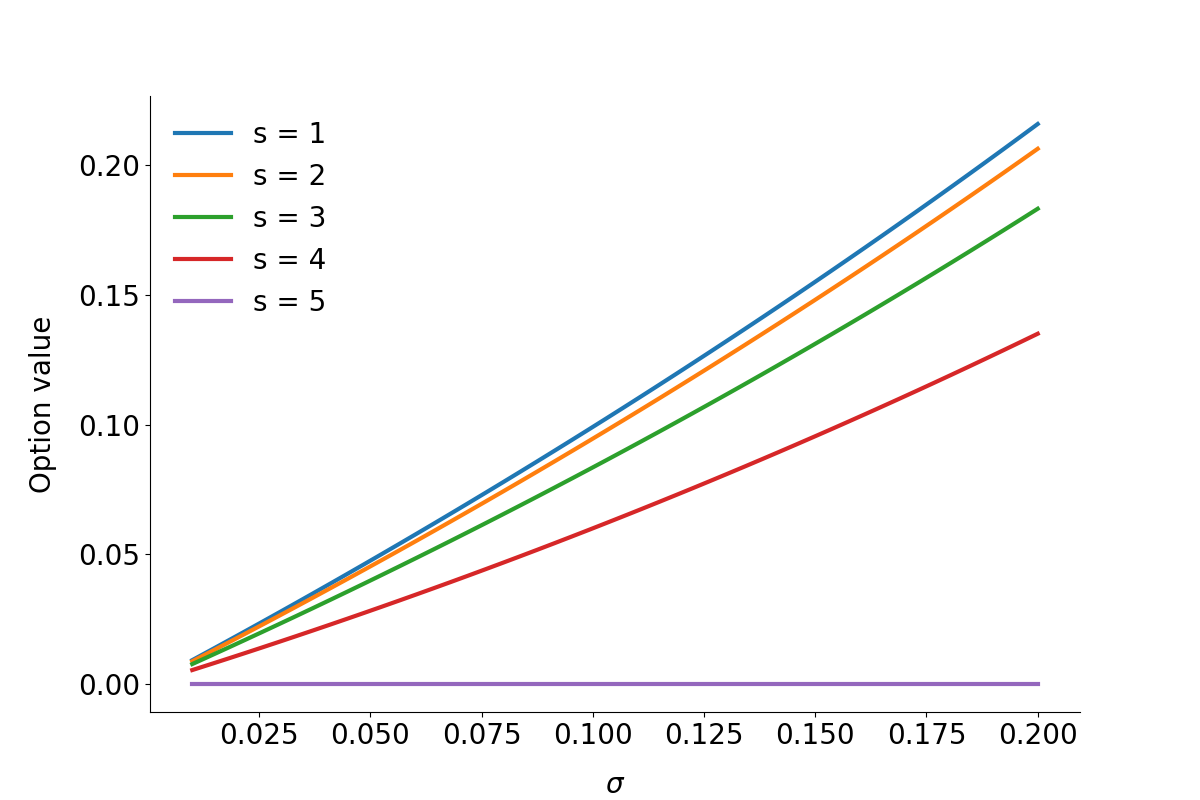
\includegraphics{fig-model-true-uncertainty}}
\end{figure}
\end{frame}
%-------------------------------------------------------------------------------
%-------------------------------------------------------------------------------
\begin{frame}
\begin{figure}[htp]\centering
\caption{Option values and nonlinearities}
\scalebox{0.35}{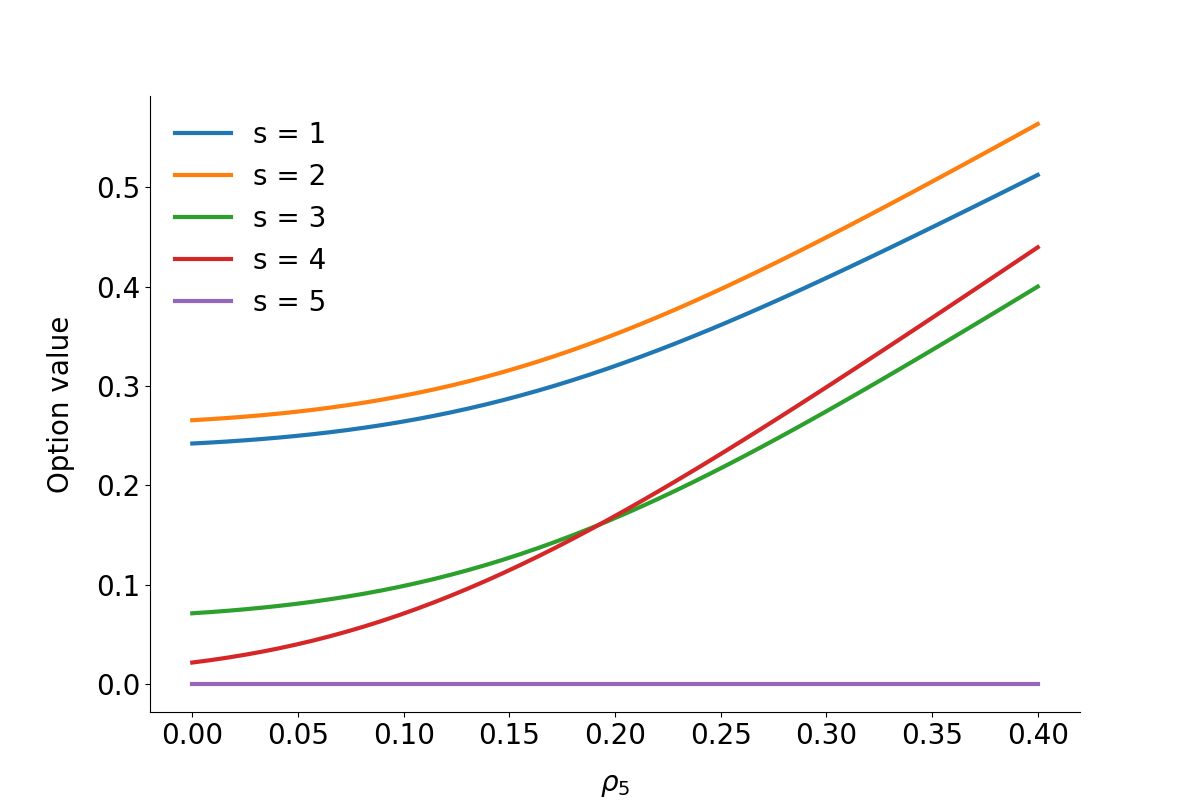
\includegraphics{fig-model-true-nonlinearities}}
\end{figure}
\end{frame}
%-------------------------------------------------------------------------------
%-------------------------------------------------------------------------------
\begin{frame}
\begin{figure}[htp]\centering
\caption{Returns}
\scalebox{0.35}{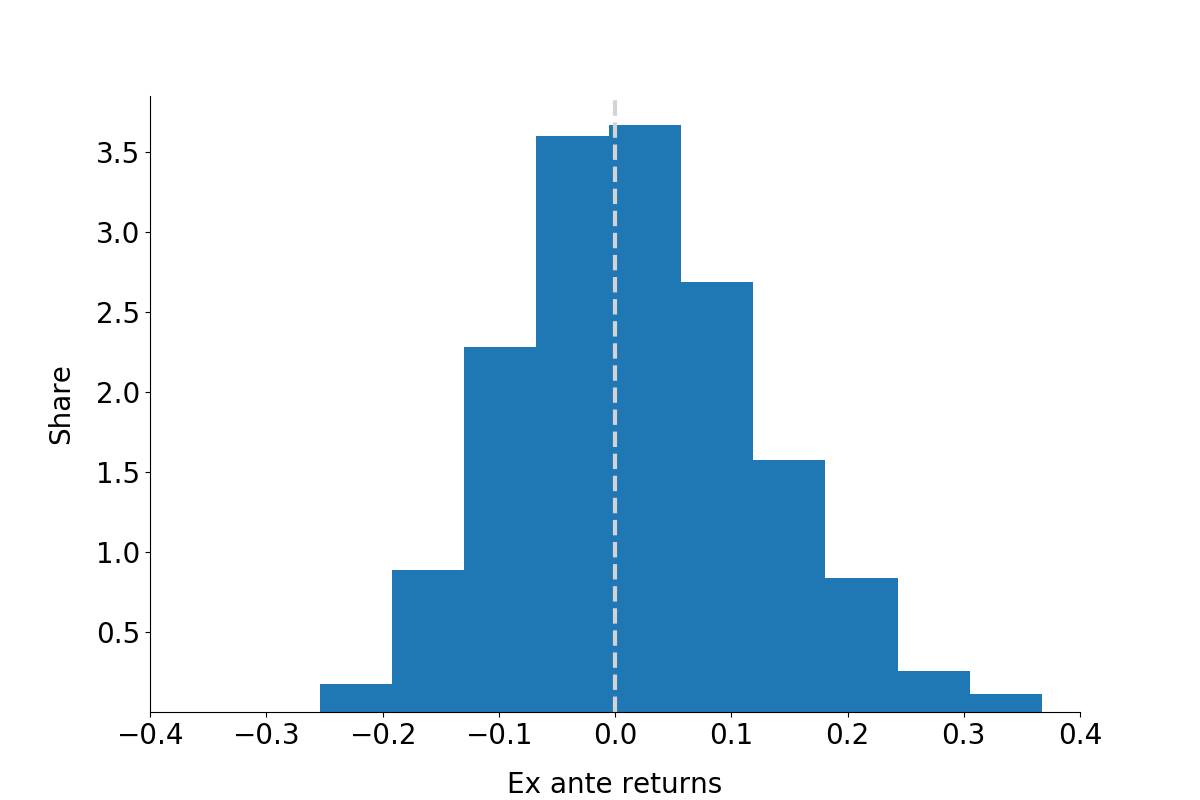
\includegraphics{fig-model-true-returns}}
\end{figure}
\end{frame}
%-------------------------------------------------------------------------------
%-------------------------------------------------------------------------------
\begin{frame}
\begin{figure}[htp]\centering
\caption{Model structure}
\scalebox{0.35}{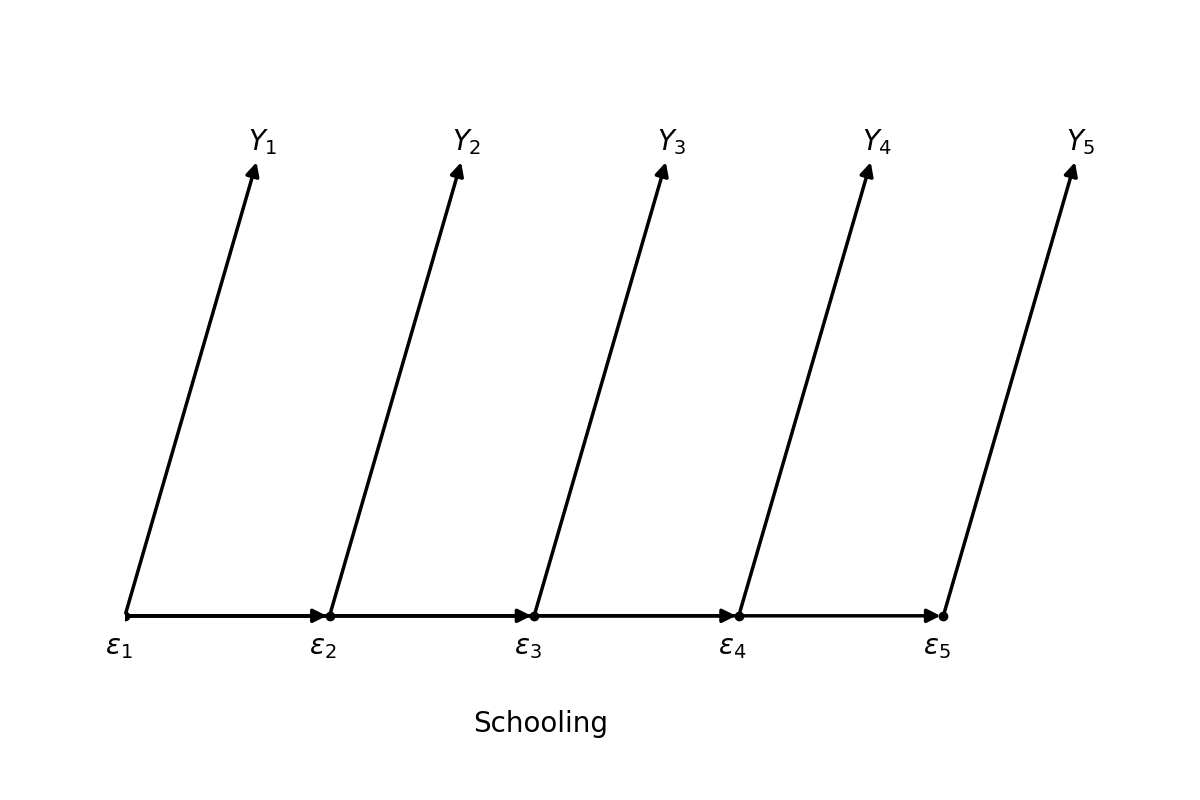
\includegraphics{fig-model-true-structure}}
\end{figure}
\end{frame}
